\documentclass[11pt,a4paper,oneside]{report}
\usepackage[tmargin=2cm, bmargin=3cm, lmargin=2cm, rmargin=2cm]{geometry}
\usepackage{helvetica}
\usepackage{tikz}
\usepackage{pgf-umlcd}
\usepackage{rotating}

\begin{document}

\title{Othello}

\maketitle

\section*{Introduction}
This report details our implementation of the game Othello, written in Java. In the report we will discuss the design decisions we made when writing the code for the game, and the reasons for these decisions. We will run through all the classes used in the solution, and explain how they are linked together using UML.

\section*{Implementation}
We implement this game using the MVC arcitecture. We decided this would be the best approach as we wanted to implement a very simple console based view, and using MVC would keep coupling between the view and the actual game data to a minimum, allowing a more advanced visual representation of the board to be pluged straight in at a later date.

\section*{The Classes}

\subsection*{Diagrammatically}
The UML diagram on the next page shows the relationships between the classes in our implementation.

\begin{sidewaysfigure}
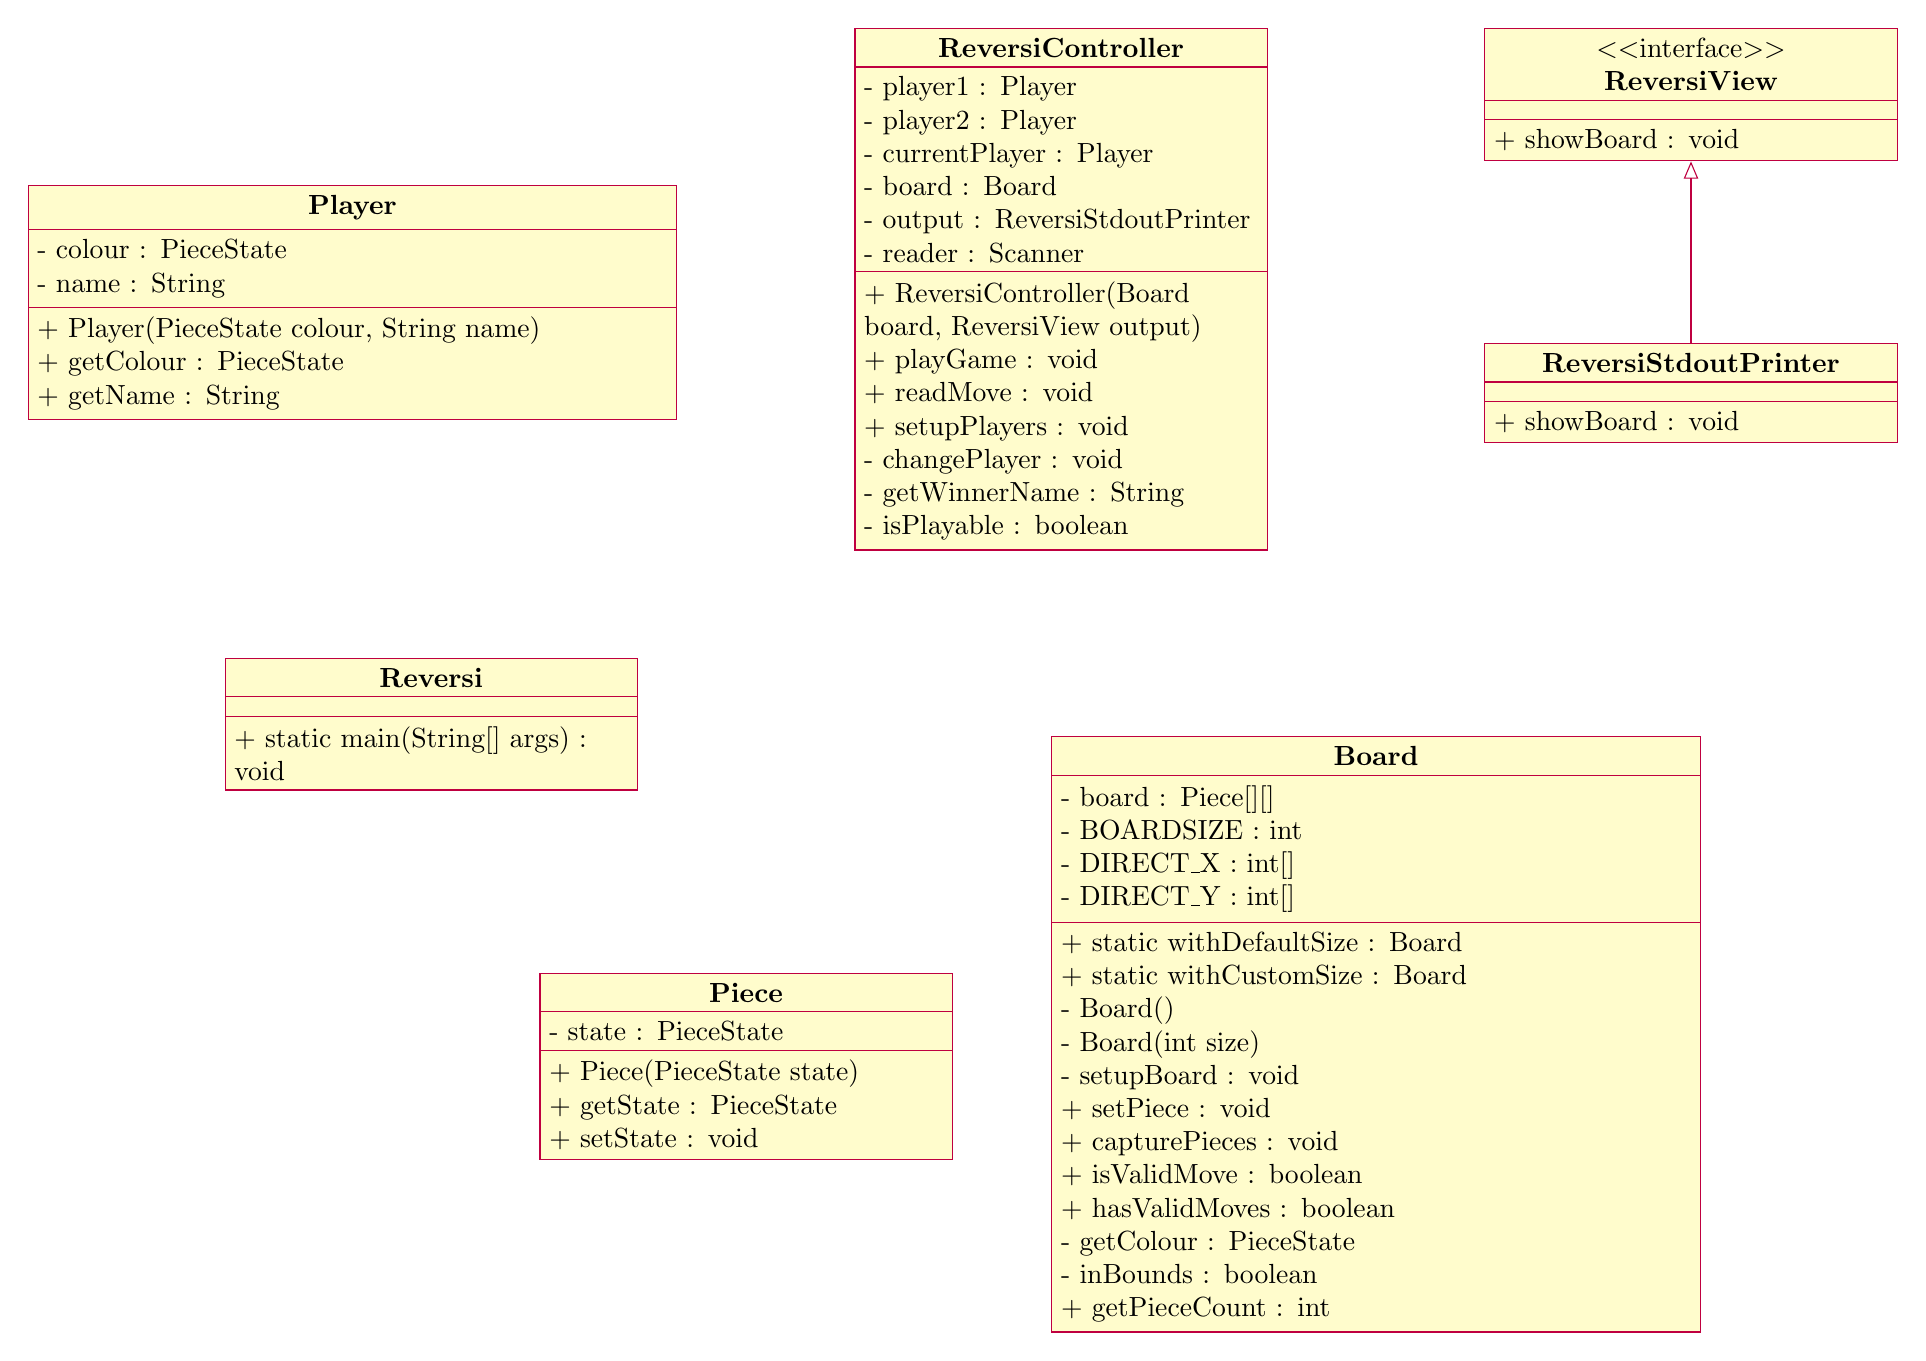
\begin{tikzpicture}
\begin{class}{ReversiController}{12,16} 
\attribute{- player1 : Player}
\attribute{- player2 : Player}
\attribute{- currentPlayer : Player}
\attribute{- board : Board}
\attribute{- output : ReversiStdoutPrinter}
\attribute{- reader : Scanner}
\operation{+ ReversiController(Board board, ReversiView output)} 
\operation{+ playGame : void}
\operation{+ readMove : void}
\operation{+ setupPlayers : void}
\operation{- changePlayer : void}
\operation{- getWinnerName : String}
\operation{- isPlayable : boolean}
\end{class}

\begin{class}[text width=8cm]{Board}{16,7}
\attribute{- board : Piece[][]}
\attribute{- BOARDSIZE : int}
\attribute{- DIRECT\_X : int[]}
\attribute{- DIRECT\_Y : int[]}
\operation{+ static withDefaultSize : Board}
\operation{+ static withCustomSize : Board}
\operation{- Board()}
\operation{- Board(int size)}
\operation{- setupBoard : void}
\operation{+ setPiece : void}
\operation{+ capturePieces : void}
\operation{+ isValidMove : boolean}
\operation{+ hasValidMoves : boolean}
\operation{- getColour : PieceState}
\operation{- inBounds : boolean}
\operation{+ getPieceCount : int}
\end{class}

\begin{interface}{ReversiView}{20,16}
\operation{+ showBoard : void}
\end{interface}

\begin{class}{ReversiStdoutPrinter}{20,12}
\inherit{ReversiView}
\operation{+ showBoard : void}
\end{class}

\begin{class}[text width=8cm]{Player}{3, 14}
\attribute{- colour : PieceState}
\attribute{- name : String}
\operation{+ Player(PieceState colour, String name)}
\operation{+ getColour : PieceState}
\operation{+ getName : String}
\end{class}

\begin{class}{Piece}{8,4}
\attribute{- state : PieceState}
\operation{+ Piece(PieceState state)}
\operation{+ getState : PieceState}
\operation{+ setState : void}
\end{class}

% not sure how to do this
%
% \begin{umlenum}{PieceState}{0,0}
% \attribute{EMPTY}
% \attribute{WHITE}
% \attribute{BLACK}
% \end{umlenum}

\begin{class}{Reversi}{4,8}
\operation{+ static main(String[] args) : void}
\end{class}

\end{tikzpicture}
\end{sidewaysfigure}

\subsection*{Reversi}
This class acts as the entry point for the program. The only thing this class does is instantiate the Model, View and Controller, and checks to make sure the command line arguments (if any) are valid. Then it calls the controller to start the game.

\subsection*{ReversiController}
The controller manages the game. It creates the two players, gives them names and colours, and keeps track of which player can go in the current turn. It starts the game, reading in moves from stdin and converting them to integer input which it then uses to manipulate the model (the part of the model it accesses is the Board class). After each moves it checks if the game is over. If it isn't then it reads the next move from the other player, if it is then it declares the winner.

\subsection*{Player}
This simple class keeps track of the player's name and colour. These private fields are encapsulated and getters are provided for them (as is the case throughout the project).

\subsection*{Board}
This class is the basis of the model in the program. It holds the data structure representing the game board itself (in the form of a 2D array of Piece objects), and provides methods to manipulate the data structure: it can get and set the state of pieces in the board, check if a move is valid, check if a Piece of a certain colour can be played anywhere on the board, flip the pieces that should be flipped once a piece has been played, and count the number of pieces of a particular colour on the board.\\
\indent The Board class can be constructed in multiple ways - with a single integer argument which denotes the size of the board, or without any arguments (in which case the default size of 8 is used). We implemented this using the Factory pattern, as originally it was not at all clear what the constructor with the integer did without delving into the class definition. For this Factory pattern we defined two static methods, called \texttt{withDefaultSize()} and \texttt{withCustomSize(int size)}, which insantiate the private contructors \texttt{Board()} and \texttt{Board(int size)} respectively. In both contructors, the board is then set up with the four central pieces filled with alternating tiles (this rule is specific to Othello and not used in Reversi). 

\subsection*{Piece}
This class represents a piece that can be placed on the board. It holds a field which represents the colour of the piece (either BLACK, WHITE or EMPTY). The class provides a getter and a setter for this field, which can be used when flipping a piece on the board. 

\subsection*{PieceState}
This enumeration is used by the Piece class to store it's colour, and also by the Player class, to store which colour each player is playing with. We used the one enum for both to ensure the avoidance of uneccessary code duplication.

\subsection*{ReversiView}
This interface can be implemented by any concrete view of the game, in order to easily plug in to the model and the controller. It has one method, \texttt{showBoard(Board)}, which can be used by a view implementing the interface to print or refresh the board in whichever way it chooses.

\subsection*{ReversiStdoutPrinter}
This is our chosen implementation of the ReversiView interface. It prints the board to the console, with row numbers and column letters. It uses dots for empty spaces and W and B for the colours.

\end{document}
